\documentclass[]{spie}  %>>> use for US letter paper
%\documentclass[a4paper]{spie}  %>>> use this instead for A4 paper
%\documentclass[nocompress]{spie}  %>>> to avoid compression of citations

\renewcommand{\baselinestretch}{1.0} % Change to 1.65 for double spacing
 
\usepackage{amsmath,amsfonts,amssymb}
\usepackage{graphicx}
\usepackage{algorithm}
\usepackage[noend]{algpseudocode}
\usepackage[colorlinks=true, allcolors=blue]{hyperref}
\newcommand{\mycomment}[1]{}

\title{2D ISAR Modified Orthogonal Matching Pursuit for Doppler-Ambiguous and Off-grid Target Scatterers}

\author[a]{Brandon Boucher}
\author[b]{Mike Davis}
\author[b]{Greg Showman}
\author[b]{Dan Cook}
\author[a]{Justin Romberg}
\affil[a]{Georgia Institute of Technology, 225 North Avenue, Atlanta, US}
\affil[b]{Georgia Tech Research Institute, 250 14th Street, Atlanta, US}

\authorinfo{Further author information: (Send correspondence to Brandon Boucher)\\Brandon Boucher: E-mail: bboucher9@gatech.edu, Telephone: 1 720 443 8892\\  B.B.A.: E-mail: bba@cmp.com, Telephone: +33 (0)1 98 76 54 32}

% Option to view page numbers
\pagestyle{empty} % change to \pagestyle{plain} for page numbers   
\setcounter{page}{301} % Set start page numbering at e.g. 301
 
\begin{document} 
\maketitle

\begin{abstract}
Inverse Synthetic Aperture Radar (ISAR) imaging is advantageous to surveillance and reconnaissance efforts as it enables imaging in any weather, day or night. However, the resolution of the image is dependent on angular diversity and is susceptible to errors from the higher-order motion parameters of a non-cooperative target. For example, if the pulse repetition frequency (PRF) is insufficient to process the incoming Doppler bandwidth of the received echoes, the image can have aliased scatterers. Additionally, target scatterers rarely fit to a defined grid typically used for ISAR imaging, which creates matching basis errors. Though existing methods in literature have demonstrated good reconstruction quality, many have inherent limitations. Learning-based methods require training which can be difficult for ISAR imaging as publicly available real data is scarce. Other methods, like sparse Bayesian learning (SBL) and atomic norm minimization (ANM), are computationally burdensome which can be disadvantageous for imaging platforms with hardware and software limitations or in scenarios where real-time imaging is paramount. Our proposed solution, a modified Orthogonal Matching Pursuit (OMP) algorithm, is able to use the non-uniform motion of the target to aid in disambiguating target scatterers, and our algorithm efficiently finds off-grid target scatterers through Newton’s method. Our algorithm identifies aliased targets in an unambiguous region and determines the originating ambiguity by assessing the correlation of each ambiguous atom with the residual. Our modified OMP processes the latent image in a singular ambiguity as opposed to expanding the sensing matrix to incorporate other ambiguities. This reduces the sensing dictionary dimensionality. From the estimated scattering position, our algorithm then applies Newton’s method in a local neighborhood to refine the off-grid position. Preliminary results demonstrate the algorithm’s effectiveness relative to other modified OMP algorithms, outperforming each in positional accuracy and computational burden.
\end{abstract}


% Include a list of keywords after the abstract 
\keywords{ISAR, doppler ambiguity, non-uniform motion, off-grid}

\section{INTRODUCTION}
\label{sec:intro}  % \label{} allows reference to this section

% ------------------- motivation, Doppler ambguity ------------------

% This paragraph introduces ISAR imaging as well as Doppler ambiguities with an example of where Doppler ambiguities can effect an image

% motivation and Doppler ambiguity
Inverse synthetic aperture radar (ISAR) imaging enables image creation in all weather at any time of the day or night. The range resolution of an ISAR image is dependent on the bandwidth of the radar, and the crossrange resolution is dependent on the angular diversity of the target. As the target rotates and the integration angle increases or the radar has more looks at a target, the crossrange resolution improves and scatterers are more easily differentiated. However, for non-cooperative targets, the target's motion is typically complex and has high-order motion parameters, rotational acceleration, jerk, etc \cite{Liu_2012}. This complex motion can result in Doppler aliasing. Doppler aliasing or Doppler ambiguity arrises when the PRF is less than twice the Doppler frequency of a scatterer. This is a common occurance in applications like space surveillance and imaging of group targets where the far distances necessitates a low PRF or the extension of the target exceeds the Doppler bandwidth [\citenum{Huang2016, Liu2022}]. The result is ambiguous Doppler frequencies fold into the unambiguous region where Doppler frequencies originating from ambiguous and unambiguous regions can no longer be differentiated. 

% --------------- SAR Doppler ambiguity literature review --------------

% I think this paragraph could speak to the plethora of different methods available for Doppler ambiguity removal. 

% To do:
% 1. find a survey that walks through all of the different DAR methods

In SAR imaging, there are a variety of different well-known and well-researched methods for handling Doppler ambiguity of a Doppler centroid. These methods are valuable but Doppler ambiguity arrises differently in ISAR compared to SAR, and alternative ISAR-specific Doppler ambiguity resolver methods are worth exploring. 

% ------------- ISAR Doppler ambiguity literature review ------------

% This paragraph reviews the current ISAR Doppler ambiguity literature

% To do:
% 1. continue searching for competing methods:
%   isar doppler ambiguity
%   isar group targets
%   isar doppler aliasing
%   check citations of Huang and Liu again

However, literature directly investigating resolving or removing ISAR Doppler ambiguity for extended or group targets is more scarce. The available literature is primarily focused on leveraging migration through range cells (MTRC) in order to differentiate ambiguous and unambiguous scatterers. The authors of [\citenum{Huang2016}] applying OMP to form an image by removing the Doppler ambiguity and correcting range cell. Their method leverages the differences in phase progression resulting from range-azimuth coupling and applies OMP to each range cell selecting Fourier-based atoms as a function of Doppler frequency, chirp rate and Doppler ambiguity. Using the selected atoms and subsequently estimated signal parameters, their method removes the Doppler ambiguity and corrects for range cell migration. This method effectively removes Doppler ambiguity; however, their method assumes uniform motion, the scatterers are on-grid, and their method relies on range-azimuth coupling in order disambiguate atoms. Additionally, because the Doppler ambiguity is included as a dimension in their sensing matrix, the dimensionality and complexity far exceeds our proposed method. The authors of [\citenum{Liu2022}] use maximum weighted contrast to compare the range-walk produced by the estimated motion parameters and the range-walk for each ambiguity. The correct ambiguity corrects the range-walk and the scatterer's peak sharpens. [\citenum{Liu2022}] applies a Gaussian weighting to mitigate the sidelobes of the echo where the standard deviation is proportional to the standard deviation of the data in each range cell [\citenum{Liu2022}]. Their method is an effective approach in addressing Doppler ambiguity, but assumes each range cell contains a singular scatterer and suffers from on-grid approximation in determining position.

% --------------- Off-grid introduction and literature review --------------

% I think this paragraph should start by mentioning the above methods do not assume off-grid, and then I think it should transition into a brief literature review of off-grid methods.

% To do:
% 1. learning-based methods citations
% 2. find other OMP off-grid methods

Another assumption common in both [\citenum{Huang2016,Liu2022}] is the scatterers fall on-grid, dependent on the range and azimuth sampling. However, real targets do not fall perfectly inline with pre-defined grids, and this descrepancy can cause distortion errors resulting from basis mismatch [\citenum{chi2011}]. The obvious fix is to increase the number of grid points, thereby distributing the energy of the measured reflectivity in a more exact position. This method has drawbacks, and is typically limited by both the additional computation required by increasing the dimensionality of the problem and by the increase in the coherence of atoms if using CS methods. Modern off-grid imaging methods like sparse Bayesian learning (SBL) [\citenum{Tipping2001,Ji2008,Liu2014,Xiong2025}] and atomic norm minimization (ANM) [\citenum{Chandrasekaran2012,tang2013,Yang2016,Mingjiu2022}] are inherently continuous, enabling state-of-the-art reconstruction. However, SBL and ANM are computational expensive and are not feasible for on-board image processing.  In the pursuit of a real-time, off-grid ISAR image former, several authors have modified OMP. Most notably, Newtonized OMP (NOMP) cyclically refines each estimated target scatterering position individually using Newton's method [\citenum{Mamandipoor2015}]. Parameter-Refined OMP (PROMP) jointly refines the target scattering positions and reflectivities by calculating a Jacobian of the combined state [\citenum{Nguyen2019}].

\mycomment{Learning-based methods like unfolding networks substitute the steps of iterative algorithms with neural networks where computation is reduced to single passes through neural layers. However, learning-based methods are only as good as their training data, and publicly available ISAR data is scarce. Many of the learning-based implementations then must train on small datasets and synthetic data which degrades generalizability.}

\subsection{Contributions}

% non-uniform phase progression -> atom differentiation
Traditionally higher-order motion parameters are seen as a nuisance as they can corrupt and contaminate the image formation process with unwanted phase errors. Higher-order motion parameters also introduce non-uniform phase progression and migration through range cells (MTRC). The goal of this paper is to leverage non-uniform phase progression from non-uniform motion to differentiate unambiguous and ambiguous target scatterers. Additionally, our formulation of the problem naturally enables off-grid scatterer compensation where we apply Newton's method to a local neighborhood surrounding a candidate atom. Our key contributions are:

\begin{enumerate}
    \item Our proposed method, AROMP is capable of differentiating Doppler ambiguous scatterers by leveraging the non-uniform phase progression resulting from the non-uniform rotation of the target
    \item We perform off-grid reconstruction using Newton's method within a neighborhood of ambiguous and unambiguous candidate atoms
    \item We define a performance metric by which we can compare the outputs of ISAR images with strong individual scatterers.
\end{enumerate}

\section{BACKGROUND}

ISAR imaging requires translational motion compensation and rotational motion compensation. Translational motion compensation is typically regarded as trivial and does not add anything outside of undesirable blurring. Assuming the translational motion compensation has been appropriately applied, Figure \ref{fig:geo} depicts the geometry of the target during ISAR imaging where the target is rotating between pulses.

\subsection{Target Geometry}

The crossrange resolution of ISAR images is dictated by the rotation of the target. Assuming translational motion compensation has been applied, this reduces the ISAR model to a tabletop, where the target rotates at a fixed position away from the radar. Additionally, for the purposes of specifically evaluating the effects of non-uniform sampling and slow-time undersampling, the rotation motion parameters are assumed to be known. Figure \ref{fig:geo} depicts the ISAR imaging geometry.

\begin{figure}[h]
  \centering
  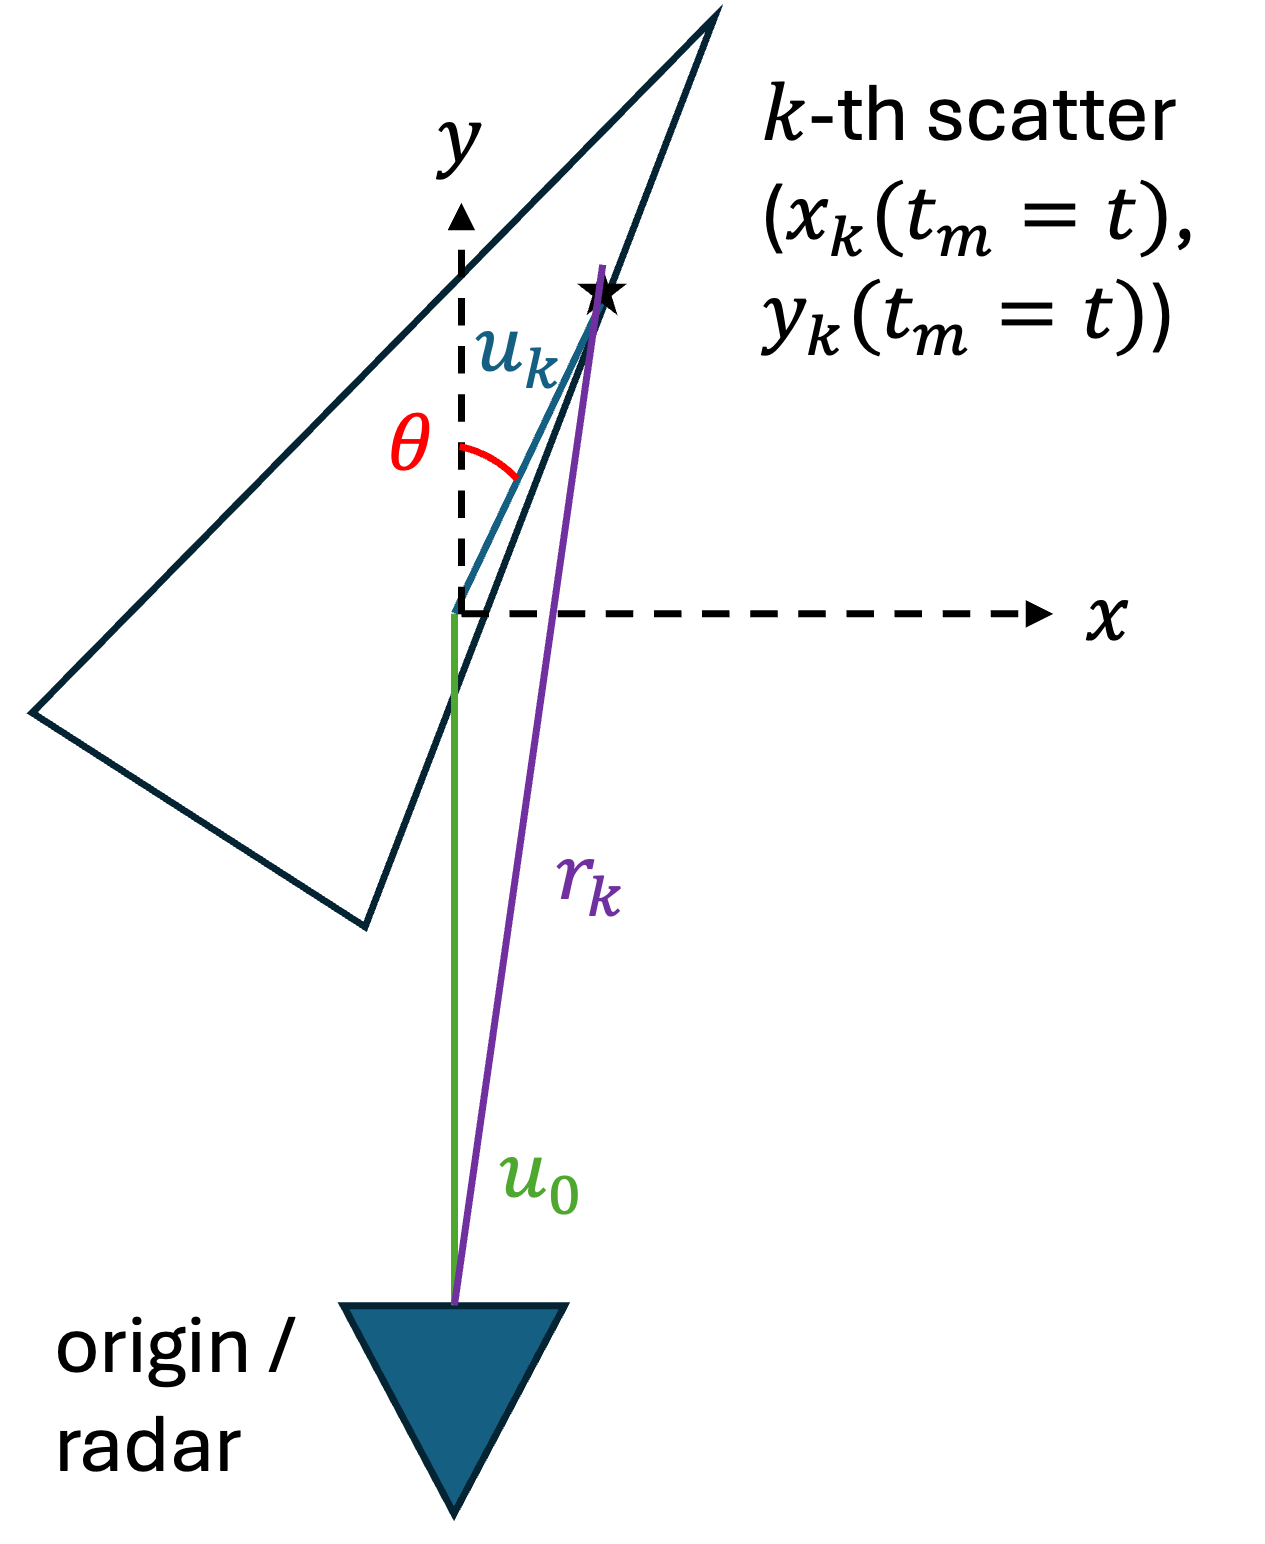
\includegraphics[width=0.3\linewidth]{figures/isar_geo2.png}
  \caption{ISAR target geometry as a function of slow-time}
  \label{fig:geo}
\end{figure}

\noindent The relative position of a scattering point as a function of slow-time ($t_{m}$) can be defined as \cite{Xu2022}:

\begin{equation}
    \begin{bmatrix}
        x_{k}(t_m)\\
        y_k (t_m)
    \end{bmatrix}
    =
    \begin{bmatrix}
        \cos(\theta(t_m)) & -\sin(\theta(t_{m})) \\
        \sin(\theta(t_m)) & \cos(\theta(t_m))
    \end{bmatrix}
    \begin{bmatrix}
        x_{k}\\
        y_k
    \end{bmatrix}
\end{equation}


\noindent where $\theta(t_{m})$ or $\theta_m$ is the angle of the target scatterer relative to the $y$-axis, and $[x_{k}, y_{k}]^{T}$ is the initial position of the $k$-th scatterer relative to the center of the rotation of the target. The range from the origin located at the radar to a scattering point is \cite{Xu2022}:
\begin{equation}
    \begin{aligned}
        r_{k}(t_m) &= \sqrt{x_{k}^2(t_m) + (y_k(t_{m}) + u_{0})^2}\\
        &\approx u_{0} + y_{k}(t_m) \quad \mathrm{as} \quad (y_k(t_{m}) + u_{0})^2 >> x_{k}^2(t_m)\\
        &= u_{0} + x_{k} \sin(\theta(t_{m})) + y_{k}\cos(\theta(t_{m}))\\
        &= u_{0} + u_{k} \\ &\mathrm{where} \quad u_{k} = x_{k} \sin(\theta(t_{m})) + y_{k}\cos(\theta(t_{m}))
    \end{aligned} 
    \label{eq:r}
\end{equation}

\noindent The angle $\theta_m$ can be approximated using a Taylor series:

\begin{equation}
    \begin{aligned}
        \sin(\theta) &= \theta - \frac{\theta^3}{3!} + \frac{\theta^{5}}{5!} + \dots \\
        \cos(\theta) &= 1 - \frac{\theta^2}{2!} + \frac{\theta^{4}}{4!} + \dots
    \end{aligned}
\end{equation}

\noindent For most ISAR applications, the target's rotation is relatively small across the coherent integration time, enabling the usage of the small angle approximation: $\sin(\theta(t_{m})) \approx\theta(t_{m})$ and $\cos(\theta(t_m)) \approx 1$. The range from the radar to a target scatterer can be approximated as:

\begin{equation}
  \begin{aligned}
    r_{k}(t_{m}) &\approx u_{0} + y_{k} + x_{k}\theta_{m} \\ \theta(t_{m}) &= \theta(0) + \omega t_{m} + \frac{\dot{\omega}}{2}t_{m}^{2} + \dots
  \end{aligned}
  \label{eq:r_final}
\end{equation}

\subsection{Signal Model and Sensing Matrix} \label{sec:signal} 

% target geometry
 The signal can be represented as a range-compressed echo:

\begin{equation}
    s(\hat{t},t_{m}) = C \cdot \text{sinc}(B(\hat{t} - \tau(t_{m})))\cdot \exp(-j2 \pi f_{c} \tau(t_{m}))
\end{equation}

\noindent where $C$ is the amplitude, $B$ is the bandwidth, $\hat{t}$ is the fast-time, $t_{m}$ is the slow-time, $\tau$ is the propagation delay and $f_{c}$ is the center frequency. The propagation delay for a monostatic radar configuration is the amount of time required to propagate to the target and return:

\begin{equation}
    \tau_{m} = \frac{2r(t_{m})}{c}
\end{equation}

\noindent where $r(t_{m})$ is the range or distance from the radar to a target scattering point as defined by equation \ref{eq:r}. The return echo can be represented as a summation of the returns from each scatterer:

\begin{equation}
    s(\hat{t},t_{m}) = C \sum_{k} \sigma_{k} \cdot \delta(\hat{t} - \tau_{k}(t_{m})) \cdot \exp(-j2 \pi f_{c} \tau_{k}(t_{m}))
\end{equation}

\noindent where $k$ is the index of each scatterer located at $\delta(\hat{t} - \tau_{k}(t_{m}))$, $K$ is the total number of scatterers or sparsity, and $\sigma_{k}$ is the complex reflectivity of the $k$-th scatterer. Typical formulations will assume separability in the range and crossrange to simplify the sensing matrix's formulation; however, this approach neglects the cross-terms inherent to range-cell migration. To preserve this effect while still defining a linear system suitable for reconstruction using compressed sensing, apply the Fourier transform in the fast-time:

\begin{equation}
    S(\hat{f},t_{m}) = C \sum_{k} \sigma_{k} \cdot \exp(-j2 \pi (f_{c} + \hat{f}) \tau_{k}(t_{m}))
    \label{eq:S}
\end{equation}

\noindent where $\hat{f}$ is the temporal-frequency or the range-frequency. Equation \ref{eq:S} enables a formulation of a sensing matrix where each entry can be defined as:

\begin{equation}
    A[{m + \ell M}, k] = C \sigma_{k} \cdot \exp(-j2 \pi (f_{c} + \hat{f}_{\ell}) \tau_{k}(t_{m}))
\end{equation}

\noindent The resulting linear system is defined as: $y = Ax + n$, where $y \in \mathbb{C}^{ML}$ is the measurement, $A \in \mathbb{C}^{ML \times K}$ is the sensing matrix, and $x \in \mathbb{C}^{K}$ is the vectorized latent image. The dimensionality of the system is determined by the number of range-frequency samples $L$, the number of scatterers $K$ and the number of received pulses $M$ which is less than the number of total pulses $N$ such that $M << N$. Figure \ref{fig:sensing_matrix} depicts the dimensionality of the proposed sensing matrix. 

\begin{figure}[h]
  \centering
  
\includegraphics[width=0.4\linewidth]{figures/linear_sys1.png}
  \caption{Linear system formulation and dimensionality}
  \label{fig:sensing_matrix}
\end{figure}

This system is underdetermined and has infinitely many solutions, each existing in the ($N-M$)-dimensional null space of the sensing matrix. However, to treat this as a compressed sensing problem, if the latent image can be assumed $K$-sparse or containing $K$ non-zero values, the problem becomes $K$-dimensional where $M \geq K$. Additionally, if the sensing matrix is roughly orthogonal and incoherent, associated with the Restricted Isometric Property (RIP), the solution can be unique \cite{Majumdar_2018}. The compressed sensing problem can then be formulated as:

\begin{equation}
    \min_{x} ||x||_{0} \quad \text{subject to} \quad y = Ax
    \label{eq:l0}
\end{equation}

\subsection{OMP}
\label{sec:omp}
There are many different compressed sensing techniques, and Greedy algorithms like Orthogonal Matching Pursuit (OMP) are effective for non-linear recovery \cite{Bostock_2017}. For a Hermitian sensing matrix ($A$) where $A^{-1} = A^{H}$, OMP iterates through a defined sparsity ($K$) and finds the indices ($\Lambda$) that maximize the projection of the residual, initialized as the measurement, onto the basis vectors formed by $A$. The maximization of the residual selects the coefficients projected on the basis vectors formed by $A$, and the step $r = y - A \hat{X}$ prevents the re-selection of the same indices. The latent image estimation $\hat{X}$ is the least-squares approximation formed from the selected basis vectors of $A$. Algorithm \ref{algo:OMP} formally describes the OMP algorithm \cite{Majumdar_2018}.

\begin{algorithm}[H]
\caption{Orthogonal Matching Pursuit}\label{algo:OMP}
\begin{algorithmic}[1]
\Procedure{OMP}{$H,N$}
\State $\Lambda\gets []$
\State $r \gets y$
\State $\hat{X} \gets 0$
\For{$i \leq K$}
\State $c\gets A^{H}r$
\State $\Lambda = \arg\max_{i} \big| c_i \big|$
\State $\Lambda \gets \begin{bmatrix} \Lambda \\ l \end{bmatrix}$
\State $\hat{X} \gets (A(\Lambda)^{H}A(\Lambda))^{-1}A(\Lambda)^{H}y$
\State $r \gets y - A\hat{X}$
\State $i \gets i + 1$
\EndFor
\State \textbf{return} $\hat{X}$
\EndProcedure
\end{algorithmic}
\end{algorithm}

\section{Methods}
\label{sec:methods}

The intention of this section is to walk through the proposed modifications to OMP to handle Doppler ambiguities and off-grid target scatterers. Algorithm \ref{algo:AROMP} illustrates the steps of AR-OMP. AR-OMP is similar in principle to the original OMP algorithm described in Section \ref{sec:omp} where atoms are selected based on maximization with the residual. However, AR-OMP makes two distinct modifications, assessment of candidate ambiguous atoms from an initial detection in the unambiguous region and off-grid refinement. Section \ref{sec:atom_selection} reviews the candidate atom selection, \textsc{SelectCandidate} in Algorithm \ref{algo:AROMP} and detailed in Algorithm \ref{algo:candidates}. Section \ref{sec:off_grid} covers the off-grid refinement in the local neighborhoods of the ambiguous scatterers, \textsc{Refine} and \textsc{CyclicRefine} in Algorithm \ref{algo:refine}.

\begin{algorithm}[ht]
\caption{Doppler Ambiguity Refined Orthogonal Matching Pursuit (DAR-OMP)}\label{algo:AROMP}
\begin{algorithmic}[1]
\Procedure{AR-OMP}{$A, \mathbf{p}, s, K, \tau, R_c, \Delta_{c}, \Delta_{r}$}
  \Comment{dictionary of the unambiguous region, grid positions,
           measurement, sparsity, noise level, refinement cycles, crossrange search extent, range extent}
\State $\Lambda \gets \emptyset$,\; $A_s \gets [\,]$,\; $\hat{P} \gets [\,]$,\; $r \gets s$
\For{$i = 1$ \textbf{to} $K$}
  \State $c \gets A^{H}r$,\quad $c_\Lambda \gets 0$
    \Comment{mask atoms already selected}
  \State $\ell \gets \arg\max_{j}|c_j|$,\quad $\Lambda \gets \Lambda \cup \{\ell\}$
    \Comment{detection in the unambiguous region}
  \State $(a^\star, p^\star) \gets \textsc{SelectCandidate}(r,\, \mathbf{p}_\ell, \Delta_{c}, \Delta_{r})$
    \Comment{Algorithm \ref{algo:candidates}}
  \State $A_s \gets [A_s,\, a^\star]$,\quad $\hat{P} \gets [\hat{P},\, p^\star]$
  \State $\hat{\alpha} \gets (A_s^{H}A_s)^{-1}A_s^{H}s$
  \State $(\hat{P}, A_s, \hat{\alpha}) \gets \textsc{CyclicRefine}(s,\, \hat{P},\, R_c)$
    \Comment{Algorithm \ref{algo:refine}}
  \State $r \gets s - A_s\hat{\alpha}$
  \State \textbf{if} $\|r\|_2 \leq \tau$ \textbf{then break}
    \Comment{residual has reached the noise level}
\EndFor
\State \textbf{return} $\hat{\alpha},\, \hat{P}$
\EndProcedure
\end{algorithmic}
\end{algorithm}

\subsection{Ambiguous candidate atom selection}
\label{sec:atom_selection}

% This section discuss how we form the ambiguous neighborhood:
% 1. Doppler ambiguity width and range-walk
% 2. Randomized positions and refinement via correlation

% motivation for why you need a neighborhood
Because the motion parameters of the target are assumed to be known, the ambiguous doppelganger atoms of an unambiguous target scatterer are known to an extent. The ambiguous scatterers are approximately a Doppler width away from the position in the unambiguous region. Additionally, the range is approximately known and should be near the range of the unambiguous target scatterer. However, the position of the ambiguous scatterers are not percisely known as a consequence of the non-uniform motion. The non-uniform motion smears the scatterers in the alternate ambiguities. For example, a scatterer located in a -1 ambiguity is sharp with a well-defined mainlobe, but the target is progressively smeared more and more when evaluating the same scatterer at ambiguities 0, +1, +2, etc. The most straightforward method for accounting for the target smearing in other ambiguities is to expand the sensing matrix to include all other ambiguities. However, adding all ambiguities of interest increases the dimensionality of the sensing matrix from $K$ atoms to $N_{a}*K$ atoms, where $N_{a}$ is the number of ambiguities. Alternatively a more targeted approach is to evaluate only a select number of candidate atoms in alternate ambiguiites. This collection of atoms in each ambiguity will be referred to as a neighborhood. Evaluating only neighborhoods maintains the dimensionality of the sensing matrix during formation and equates to evaluating $K + N_{a}*K_{a}$ atoms, where $K_{a}$ is the number of atoms per ambiguity.

% defining the neighborhood
To define the neighborhood in the crossrange, the Doppler width can be used to search in localized regions. The Doppler width defines unambiguous and ambiguous regions and can be derived from the boundaries of the ambiguities. For a scatterer to be unambiguous, the Doppler frequency must be less than half of the PRF, $2*f_{D} < \text{prf}$, where $f_{D} = \omega \times W_{x} / \lambda$. Therefore, the Doppler width or the boundaries between ambiguities is defined as:

\begin{equation}
  \begin{aligned}
    2 f_{D} &= \text{prf} \\
    2 \omega \times W_{x} / \lambda &= \text{prf} \quad \textrm{where for a tabletop} \quad \omega \times W_{x} = \omega W_{x} \\ 
    W_{x} &= (\text{prf}) \lambda / 2 \omega
  \end{aligned}
\end{equation}

\noindent However, $\omega$ is a function of slow-time for a non-uniformly rotating target and thereby the Doppler width is also a function of slow-time. To account for the change in the Doppler width as a function of slow-time, we propose to create a neighborhood of candidate scatterers. In the crossrange direction, the extent of the neighborhood is the change in the Doppler width, $\Delta_{c} = \max(W_{x}(t_{m})) - \min(W_{x}(t_{m}))$. For each detected scatterer in the unambiguous region, the crossrange neighborhood is defined as $[x \pm n_{a}\bar{W_x} - \Delta_{c}/2, x \pm n_{a}\bar{W_x} + \Delta_{c}/2]$ where $x$ is the detected crossrange and $n_{a}$ is the ambiguity number. Ambiguous scatterers have variation in range as a consequence of range-walk [\citenum{Huang2016,Liu2022}]. Using the same principle as the crossrange neighborhood extent, the range extent is defined as the absolute value of the maximum range-walk across all scatterers, $\Delta_{r} = \max(r_{k}(t_{m})) - \min(r_{k}(t_{m}))$, where $r_{k}(t_{m})$ is the range of the $k$-th scatterer. For each detected scatterer in the unambiguous region, the range neighborhood is defined as $[y - n_{a}\Delta_{r}/2, y + n_{a}\Delta_{r}/2]$. 

% randomization of neighborhood atoms and refinement of candidate atoms

To form the neighborhood, uniformly randomize the positions of $K_a$ candidate atoms within each ambiguity. The randomization distributes the atoms evenly across the neighborhood and prevents poor, systemic initialization of atoms like a line of atoms tracing along a sidelobe. Additionally, to further reduce the number of candidate atoms evaluated, the set of candidate atoms can be refined. The set of candidate atoms forms a dictionary $A_{c} = [a_{1,1}, \dots a_{1,K_{a}}, a_{2, 1}, \dots, a_{n_{a}, k_{a}} a_{Na, K_{a}}]$ where $n_{a}$ is the ambiguity index and $k_{a}$ is the candidate atom index for a given $n_{a}$. To discard poorly placed candidate atoms, calculate the correlation of the dictionary $A_{c}$ with the residual $r$ and retain the top $K_{a}'$ atoms such that $K_{a}' < K_{a}$. Algorithm \ref{algo:candidates} depicts the candidate atom selection mechanism and refinement. 


\begin{algorithm}[ht]
\caption{Ambiguous candidate atom selection}\label{algo:candidates}
\begin{algorithmic}[1]
\Procedure{SelectCandidate}{$r,\, (x_0,y_0), \Delta_{c}, \Delta_{r}$}
  \Comment{residual, detected position in the unambiguous region, crossrange search extent, range extent}
\State $\mathcal{N} \gets \{\lceil n/2 \rceil(-1)^n : n = 0,\dots,N_a-1\}$
  \Comment{ambiguity indices, e.g. $\{-1,0,1\}$}
\For{$k = 1$ \textbf{to} $K_a$}
  \State $\delta^x_k \sim \mathcal{U}(-\Delta_c/2,\, \Delta_c/2)$,\quad
         $\delta^y_k \sim \mathcal{U}(-\Delta_r/2,\, \Delta_r/2)$
    \Comment{one offset pair per candidate, shared by every ambiguity}
\EndFor
\State $\mathcal{C} \gets \{\,(x_0 + n_a\bar{W}_x + \delta^x_k,\; y_0 + \delta^y_k)
        \;:\; n_a \in \mathcal{N},\; k = 1,\dots,K_a \,\}$
\State $A_c \gets [\,a(p)\,]_{p \in \mathcal{C}}$
  \Comment{$N_aK_a$ candidate atoms, never stored in $A$}
\State $\mathcal{C}' \gets$ the $K_a'$ positions of $\mathcal{C}$ with largest $|A_c^{H}r|$
  \Comment{screening, $K_a' = \lfloor N_aK_a/2 \rfloor$}
\State $\gamma^\star \gets -\infty$
\For{$p \in \mathcal{C}'$}
  \State $\hat{p} \gets \textsc{Refine}(r,\, p)$
    \Comment{Algorithm \ref{algo:refine}}
  \State $\gamma \gets |a(p)^{H}r|$
  \If{$\gamma > \gamma^\star$}
    \State $\gamma^\star \gets \gamma$,\; $a^\star \gets a(p)$,\; $p^\star \gets \hat{p}$
  \EndIf
\EndFor
\State \textbf{return} $a^\star,\, p^\star$
\EndProcedure
\end{algorithmic}
\end{algorithm}

\subsection{Off-grid neighborhood refinement}
\label{sec:off_grid}

% This section discusses how we optimize atoms:
% 1. Full Newton's method
%   1. motivation as to why assume the coefficient is dependent on the position
%   2. show the equations
% 2. Backtracking algorithm

After determining the set of candidate atoms $C'$, apply Newton's method to each atom to refine the off-grid position using the error surface defined in [\citenum{Mamandipoor2015}]. As derived in Section \ref{sec:omp}, the constrained objective function minimizes $\|y - Ax\|_{2}^{2}$ where S(x,p) [\citenum{Mamandipoor2015}]:

\begin{equation}
  \begin{aligned}
    \|y - Ax\|_{2}^{2} &= y^{H}y - y^{H}Ax - (Ax)^{H}y + (Ax)^{H}(Ax) \\
    &= \|y\|_{2}^{2} - 2\mathbb{R}\{y^{H}Ax\} + |x|\|A\|_{2}^{2}
  \end{aligned}
  \label{eq:yAx}
\end{equation}

Equation 

To find the error surface 

\begin{algorithm}[ht]
\caption{Off-grid refinement}\label{algo:refine}
\begin{algorithmic}[1]
\Procedure{Refine}{$r,\, p$}
  \Comment{residual, starting position; $R_s$ Newton steps, $B$ halvings}
\State $a \gets a(p)$,\quad $G \gets |a^{H}r|^{2}/(a^{H}a)$,\quad $\hat{p} \gets p$
\For{$t = 1$ \textbf{to} $R_s$}
  \State $n \gets a^{H}a$,\quad $\alpha \gets a^{H}r/n$,\quad $e \gets r - a\alpha$
    \Comment{least-squares amplitude and its residual, $a^{H}e = 0$}
  %\State $F_i \gets \Re\{\bar{\alpha}\,a_i^{H}e\}$
  %  \Comment{$a_i = \partial a/\partial p_i$, $a_{ij} = \partial^2 a/\partial p_i \partial p_j$}
  \State $F_{i} \gets \partial G / \partial p_{i}$ \Comment{$p_1 = x, p_{2} = y$}
  %\State $H_{ij} \gets \Re\{\bar{\alpha}\,a_{ij}^{H}e\}
  %      - |\alpha|^{2}\Re\!\left\{a_i^{H}a_j - \tfrac{(a_i^{H}a)(a^{H}a_j)}{n}\right\}$
  \State $H_{ij} \gets \partial^{2} G / \partial p_{i} \partial p_{j}$
  %\State \hphantom{$H_{ij} \gets $}$+\; \tfrac{1}{n}\Re\{(a_i^{H}e)\overline{(a_j^{H}e)}\}
  %      - \tfrac{1}{n}\Re\{\bar{\alpha}[(a_i^{H}a)(a_j^{H}e) + (a_j^{H}a)(a_i^{H}e)]\}$
  %\State \textbf{if} $\operatorname{tr}H \geq 0$ \textbf{or} $\det H \leq 0$ \textbf{then break}
  %  \Comment{not a local maximum of $G$}
  \State $d \gets H^{-1}F$,\quad \textit{accepted} $\gets$ \textbf{false}
  \For{$b = 0$ \textbf{to} $B$}
    \State $p' \gets \hat{p} - 2^{-b}d$,\quad
           $a' \gets a(p')$,\quad $G' \gets |a'^{H}r|^{2}/(a'^{H}a')$
    \If{$G' > G$}
      \State $\hat{p} \gets p'$,\; $a \gets a'$,\; $G \gets G'$,\;
             \textit{accepted} $\gets$ \textbf{true};\; \textbf{break}
        \Comment{backtracking line search}
    \EndIf
  \EndFor
  \State \textbf{if not} \textit{accepted} \textbf{then break}
\EndFor
\State \textbf{return} $\hat{p}$
\EndProcedure
\Statex
\Procedure{CyclicRefine}{$s,\, \hat{P},\, R_c$}
  \Comment{re-refine every atom selected so far}
\For{$c = 1$ \textbf{to} $R_c$}
  \For{$j = 1$ \textbf{to} $|\hat{P}|$}
    \State $r_j \gets s - A_{s,\backslash j}\,\hat{\alpha}_{\backslash j}$
      \Comment{measurement minus the other atoms}
    \State $\hat{p}_j \gets \textsc{Refine}(r_j,\, \hat{p}_j)$,\quad
           $A_{s,j} \gets \vartheta(\hat{p}_j)$
  \EndFor
  \State $\hat{\alpha} \gets (A_s^{H}A_s)^{-1}A_s^{H}s$
\EndFor
\State \textbf{return} $\hat{P},\, A_s,\, \hat{\alpha}$
\EndProcedure
\end{algorithmic}
\end{algorithm}
 


%\subsection{Complexity}
%\label{sec:complexity}

% I actually don't know that we need to include a complexity section if I just report the dictionary building plus algorithm time.

\section{Results}
\label{sec:results}

Section \ref{sec:coherence} reviews the effects of non-uniform phase progression on the coherence of the unambiguous and ambiguous atoms. Section \ref{sec:rmse} compares the positional and coefficient root mean squared error relative to other OMP-based algorithms used for off-grid imaging and Doppler ambiguity correction.

\subsection{Non-uniform sampling coherence}
\label{sec:coherence}

As mentioned in Section \ref{sec:methods}, non-uniform motion and subsequently, non-uniform phase progression is often seen as a hinderance. Non-uniform motion can introduce phase errors if not approximated and compensated for correctly. However, there is a plethora of literature on translational motion compensation, rotational motion compensation, and autofocus literature capable of target motion estimation. If the motion parameters are assumed to be known, they provide valuable information which can be leveraged to differentiate unambiguous and ambiguous atoms. One measure of the ability to differentiate dictionary atoms is coherence. Coherence is inner product between two atoms, $a_{i}^{H}a_{j}$, and represents the similarity between those vectors. Mutual coherence is the maximum coherence between any pair of atoms and has been used as a measure of atom differntiation in CS [\textbf{cite}]. The mutual coherence is the coherence between atoms within the sensing matrix, and is defined as:

\begin{equation}
    M = \max_{0 \leq i \neq j \leq K-1} |a^{H}_{i}a_{j}|
\end{equation}

To characterize and quantify the amount of help non-uniform phase progression provides, the mutual coherence of the sensing matrix was calculated as a function of the motion parameters.

\subsection{RMSE}
\label{sec:rmse}

To test the effectiveness of Doppler ambiguity and , 

\subsection{Noise assessment}
\label{sec:noise}

\section{discussion}
\label{sec:discussion}
\input{sections/conclusion.tex}


% References
\bibliography{bib} % bibliography data in report.bib
\bibliographystyle{spiebib} % makes bibtex use spiebib.bst

\end{document} 
